\section{Presnopy, snopy i topologie Grothendiecka}\label{cat:sec:grothendieck-topologies}

Snop opisuje dane lokalne oraz reguły ich jednoznacznego sklejania. Na przestrzeni topologicznej lokalność wyznaczają pokrycia otwarte. W kategorii ogólnej zastąpimy je rodzinami morfizmów stabilnymi względem składania. Wykorzystamy lemat Yonedy (twierdzenie~\ref{cat:thm:yoneda-contra}) oraz punktowe granice i kogranice (twierdzenie~\ref{cat:thm:pointwise-limits}). Klasyczne snopy, źdźbła i przykłady geometryczne omówiono w \atlasref{ALG-04::def:snop}{geometrii algebraicznej}; tutaj nacisk kładziemy na konstrukcje kategorialne, także bez przestrzeni punktów.

\subsection{Kategoria presnopów}

\begin{definicja}[Presnop zbiorów]\label{cat:def:presheaf}
Niech $\mathcal C$ będzie małą kategorią. Presnopem na $\mathcal C$ nazywamy funktor $F:\mathcal C^{\op}\to\Set$. Morfizmy presnopów to transformacje naturalne. Piszemy
\[
\widehat{\mathcal C}=[\mathcal C^{\op},\Set].
\]
Dla $f:V\to U$ i $s\in F(U)$ oznaczamy $F(f)(s)$ także przez $s|_f$. Wtedy $s|_{\id_U}=s$ i $(s|_f)|_g=s|_{fg}$.
\end{definicja}

Małość kategorii zapewnia, że rodziny składowych transformacji tworzą zbiory. Wszystkie używane dalej produkty, rodziny sit i klasy równoważności są zbiorami. Jeżeli $\mathcal C$ jest jedynie lokalnie mała, trzeba osobno ustalić warunki małości lub przejść do odpowiedniego większego uniwersum.

\begin{stwierdzenie}[Presnopy reprezentowalne]\label{cat:prop:presheaf-representables}
Dla $U\in\Ob(\mathcal C)$ presnop $h_U=\Hom_{\mathcal C}(-,U)$ jest reprezentowalny. Zanurzenie Yonedy $h:\mathcal C\to\widehat{\mathcal C}$ jest w pełni wierne, a $\Nat(h_U,F)\cong F(U)$ naturalnie w $U$ i $F$. Wszystkie małe granice i kogranice presnopów oblicza się punktowo.
\end{stwierdzenie}
\begin{proof}
Dla dowolnych $g:W\to V$ i $k:V\to U$ mamy $h_U(g)(k)=kg$. Lemat Yonedy~\ref{cat:thm:yoneda-contra} daje bijekcję $\Nat(h_U,F)\cong F(U)$, a jej naturalność w obu argumentach wynika z twierdzenia~\ref{cat:thm:yoneda-natural}. Dla $F=h_V$ otrzymujemy $\Nat(h_U,h_V)\cong\Hom(U,V)$. Bijekcja identyfikuje morfizm $U\to V$ z transformacją daną składaniem z lewej, więc zachowuje identyczności i składanie. Ostatnie stwierdzenie wynika z twierdzenia~\ref{cat:thm:pointwise-limits}, ponieważ $\Set$ ma wszystkie małe granice i kogranice.
\end{proof}

\subsection{Sita i zgodne rodziny}

\begin{definicja}[Sito]\label{cat:def:sieve}
Sitem $R$ na $U$ nazywamy podfunktor $R\subseteq h_U$. Równoważnie jest to rodzina morfizmów o przeciwdziedzinie $U$, taka że jeżeli $f:V\to U$ należy do $R$, to dla każdego $g:W\to V$ także $fg$ należy do $R$.
Sito maksymalne to $h_U$. Dla $a:V\to U$ definiujemy sito na $V$ wzorem
\[
 a^*R(W)=\{g:W\to V:ag\in R(W)\}.
\]
\end{definicja}

\begin{stwierdzenie}\label{cat:prop:sieve-pullback}
Powyższy wzór określa sito, $(ab)^*R=b^*(a^*R)$ i $\id_U^*R=R$. Ponadto $a\in R$ wtedy i tylko wtedy, gdy $a^*R=h_V$.
\end{stwierdzenie}
\begin{proof}
Jeżeli $ag\in R$ i $k$ można złożyć z $g$, to $agk\in R$, stąd $gk\in a^*R$. Dla $b:W\to V$ i $t:T\to W$ warunek $abt\in R$ jest równoważny $bt\in a^*R$, a następnie $t\in b^*(a^*R)$. Identyczność otrzymujemy podstawiając $a=\id_U$. Jeżeli $a\in R$, to każde $ag$ należy do $R$, więc $a^*R=h_V$. Odwrotnie z maksymalności wynika $\id_V\in a^*R$, a zatem $a\in R$.
\end{proof}

Rodzina $(f_i:U_i\to U)_{i\in I}$ generuje sito składające się z wszystkich morfizmów postaci $f_i g$. Nie wymaga to istnienia iloczynów włóknistych.

\begin{center}
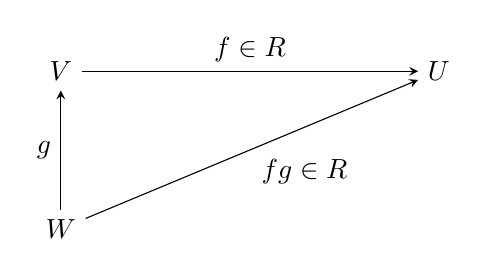
\begin{tikzpicture}[>=stealth]
 \node (w) at (0,0) {$W$};
 \node (v) at (0,2) {$V$};
 \node (u) at (4.8,2) {$U$};
 \draw[->] (w)--node[left] {$g$} (v);
 \draw[->] (v)--node[above] {$f\in R$} (u);
 \draw[->] (w)--node[below right] {$fg\in R$} (u);
\end{tikzpicture}
\end{center}

\begin{definicja}[Zgodna rodzina na sicie]\label{cat:def:matching-family}
Zgodną rodziną presnopu $F$ na sicie $R$ nazywamy transformację $x:R\Rightarrow F$. Jest to równoważnie przyporządkowanie każdemu $f:V\to U$ w $R$ elementu $x_f\in F(V)$, z warunkiem $x_{fg}=x_f|_g$ dla każdego $g:W\to V$.
\end{definicja}
Równoważność jest bezpośrednio warunkiem naturalności składowych $x_V:R(V)\to F(V)$. Każdy $s\in F(U)$ daje zgodną rodzinę $x_f=s|_f$. Na sicie maksymalnym wszystkie zgodne rodziny mają tę postać, jednoznacznie, dzięki lematowi Yonedy.

\subsection{Topologia Grothendiecka i miejsca}

\begin{definicja}[Topologia Grothendiecka]\label{cat:def:grothendieck-topology}
Topologia Grothendiecka $J$ na $\mathcal C$ przypisuje obiektowi $U$ zbiór $J(U)$ sit pokrywających, z aksjomatami:
\begin{enumerate}
\item $h_U\in J(U)$;
\item jeżeli $R\in J(U)$ i $a:V\to U$, to $a^*R\in J(V)$;
\item jeżeli $R\in J(U)$ i $S$ jest sitem na $U$ takim, że $f^*S\in J(V)$ dla każdego $f:V\to U$ w $R$, to $S\in J(U)$.
\end{enumerate}
Parę $(\mathcal C,J)$ nazywamy miejscem (ang.\ \emph{site}). Trzeci aksjomat wyraża lokalny charakter pokrywania.
\end{definicja}

\begin{lemat}[Rachunek sit pokrywających]\label{cat:lem:covering-refinement}
Niech $R,S$ będą sitami na $U$. Jeżeli $R\in J(U)$ i $R\subseteq S$, to $S\in J(U)$. Jeżeli $R,S\in J(U)$, to $R\cap S\in J(U)$. Ponadto jeśli $R$ pokrywa $U$, a dla każdego $f:V\to U$ w $R$ ustalono sito pokrywające $S_f$ na $V$, to morfizmy $fg$, $g\in S_f$, tworzą sito pokrywające $U$.
\end{lemat}
\begin{proof}
Jeśli $f\in R\subseteq S$, to $f^*S=h_V$ na mocy stwierdzenia~\ref{cat:prop:sieve-pullback}; aksjomat trzeci daje $S\in J(U)$. Dla $f\in R$ mamy $f^*(R\cap S)=h_V\cap f^*S=f^*S$, które pokrywa $V$ z aksjomatu drugiego. Ponownie stosujemy trzeci aksjomat. Rodzina złożeń tworzy sito $H$, gdyż $fgk=f(gk)$ i $gk\in S_f$. Dla każdego $f\in R$ zachodzi $S_f\subseteq f^*H$, więc z pierwszej części $f^*H$ pokrywa $V$. Aksjomat trzeci daje $H\in J(U)$.
\end{proof}

\begin{przyklad}[Miejsce przestrzeni topologicznej]\label{cat:ex:topological-site}
Dla przestrzeni $X$ bierzemy kategorię $\mathcal O(X)$ otwartych podzbiorów z morfizmami danymi przez zawieranie. Sito na $U$ jest rodziną otwartych podzbiorów $V\subseteq U$, domkniętą w dół. Uznajemy je za pokrywające, gdy $\bigcup_{V\in R}V=U$. Sito maksymalne pokrywa $U$, a przecięcie pokrycia z $W\subseteq U$ pokrywa $W$, więc zachodzą dwa pierwsze aksjomaty. Jeżeli $R$ pokrywa $U$ i $S$ pokrywa lokalnie każdy $V\in R$, to każdy $x\in U$ należy do pewnego $V\in R$, a potem do pewnego otwartego $W\subseteq V$ z $W\in S$. Zatem $S$ pokrywa $U$, także dla $U=\varnothing$.
\end{przyklad}

\begin{przyklad}[Dwie skrajne topologie]\label{cat:ex:extreme-topologies}
W topologii minimalnej jedynym sitem pokrywającym $U$ jest $h_U$. Stabilność wynika z definicji, a w aksjomacie trzecim można wziąć $f=\id_U$. W topologii maksymalnej każde sito, w tym puste, pokrywa każdy obiekt; wszystkie aksjomaty są wtedy spełnione.
\end{przyklad}

\subsection{Snopy i presnopy rozdzielone}

\begin{definicja}[Warunek snopu]\label{cat:def:site-sheaf}
Presnop $F$ jest snopem na $(\mathcal C,J)$, jeżeli dla każdego $U$ i $R\in J(U)$ odwzorowanie
\begin{equation}\label{cat:eq:sheaf-condition}
 F(U)\longrightarrow\Nat(R,F),\qquad s\longmapsto (s|_f)_{f\in R}
\end{equation}
jest bijekcją. Gdy wymagamy jedynie injektywności wszystkich tych odwzorowań, $F$ nazywamy presnopem rozdzielonym. Kategoria $\operatorname{Sh}(\mathcal C,J)$ jest pełną podkategorią $\widehat{\mathcal C}$ wyznaczoną przez snopy.
\end{definicja}

W języku Yonedy warunek snopu to bijektywność ograniczenia $\Nat(h_U,F)\to\Nat(R,F)$. Gdy puste sito pokrywa $U$, snop ma dokładnie jedną sekcję nad $U$, ponieważ z pustego funktora do $F$ istnieje dokładnie jedna transformacja naturalna. Na topologii minimalnej każdy presnop jest snopem, a na maksymalnej snopy to dokładnie presnopy o wszystkich wartościach jednoelementowych.

\begin{twierdzenie}[Zgodność z klasycznym warunkiem sklejania]\label{cat:thm:topological-sheaf-equivalence}
Na miejscu z przykładu~\ref{cat:ex:topological-site} warunek~\eqref{cat:eq:sheaf-condition} jest równoważny klasycznemu warunkowi jednoznacznego sklejania sekcji zgodnych na przecięciach elementów dowolnego pokrycia otwartego.
\end{twierdzenie}
\begin{proof}
Niech najpierw zachodzi klasyczny warunek. Dla sita pokrywającego $R$ zgodna rodzina $x_V\in F(V)$ dla $V\in R$ zgadza się na przecięciach, ponieważ $V\cap W\in R$ i oba ograniczenia są równe $x_{V\cap W}$. Klasyczne sklejanie dla pokrycia $(V)_{V\in R}$ daje jedyną sekcję nad $U$.

Odwrotnie, niech $U=\bigcup_i U_i$ i sekcje $s_i\in F(U_i)$ zgadzają się na $U_i\cap U_j$. Sito generowane przez $U_i\hookrightarrow U$ składa się z otwartych $V$ zawartych w pewnym $U_i$ i pokrywa $U$. Kładziemy $x_V=s_i|_V$, wybierając dowolne $i$ z $V\subseteq U_i$. Jeżeli także $V\subseteq U_j$, to $V\subseteq U_i\cap U_j$, więc obie wartości są równe. Dla $W\subseteq V$ ta sama sekcja $s_i$ daje $x_W=x_V|_W$. Z warunku snopu istnieje dokładnie jedna sekcja indukująca tę rodzinę, a więc ograniczająca się do $s_i$ na $U_i$. Dla pustego pokrycia otrzymujemy dokładnie jedną sekcję nad $\varnothing$, jak w definicji.
\end{proof}

\begin{definicja}[Topologia subkanoniczna]\label{cat:def:subcanonical}
Topologia $J$ jest subkanoniczna, jeżeli wszystkie presnopy reprezentowalne $h_U$ są snopami.
\end{definicja}

\begin{przyklad}[Topologia nie musi być subkanoniczna]\label{cat:ex:nonsubcanonical}
Rozważmy kategorię z dwoma obiektami $V,U$, identycznościami i jedynym nieidentycznościowym morfizmem $f:V\to U$. Na $V$ jedynym pokryciem jest sito maksymalne, a na $U$ pokrywają sita $h_U$ oraz $\{f\}$. Stabilność względem $f$ wynika z $f^*\{f\}=h_V$. Dla aksjomatu lokalnego na $U$ wystarczy zauważyć, że gdy $\{f\}$ jest sitem użytym w tym aksjomacie, warunek $f^*S=h_V$ wymusza $f\in S$, więc $S$ pokrywa. Dla sita maksymalnego stosujemy $\id_U$. Na $V$ analogicznie wystarcza identyczność. Jednak $h_V(U)=\varnothing$, podczas gdy na $\{f\}$ istnieje zgodna rodzina o jedynej wartości $\id_V\in h_V(V)$. Zatem $h_V$ nie jest snopem.
\end{przyklad}

\begin{stwierdzenie}\label{cat:prop:topological-subcanonical}
Topologia z przykładu~\ref{cat:ex:topological-site} jest subkanoniczna.
\end{stwierdzenie}
\begin{proof}
Dla otwartego $A\subseteq X$ zbiór $h_A(V)$ jest jednoelementowy, gdy $V\subseteq A$, i pusty w przeciwnym razie. Dla pokrycia $U=\bigcup_i U_i$ zgodna rodzina istnieje dokładnie wtedy, gdy każde $U_i\subseteq A$, czyli $U\subseteq A$. Gdy istnieje, jest jedyna, podobnie jak sklejona sekcja. Stosujemy twierdzenie~\ref{cat:thm:topological-sheaf-equivalence}.
\end{proof}

\begin{przyklad}[Miejsce z nietrywialnym endomorfizmem]\label{cat:ex:idempotent-site}
Niech $\mathcal C$ ma jeden obiekt $U$ i dwa morfizmy $\id_U,e$, gdzie $e^2=e$ i $e\ne\id_U$. Sita to $\varnothing,\{e\},h_U$. Przyjmijmy $J(U)=\{\{e\},h_U\}$. Stabilność wynika z $\id_U^*\{e\}=\{e\}$ i $e^*\{e\}=h_U$. W aksjomacie lokalnym dla sita maksymalnego wystarczy $\id_U$; dla $\{e\}$ warunek $e^*S\in J(U)$ wyklucza $S=\varnothing$, więc $S$ jest pokrywające.

Presnop jest tutaj zbiorem $M=F(U)$ z funkcją $p=F(e):M\to M$, spełniającą $p^2=p$. Zgodna rodzina na sicie $\{e\}$ jest wyznaczona przez $x_e=m$ z warunkiem $p(m)=m$, ponieważ $ee=e$. Ograniczenie sekcji do tego sita jest więc funkcją
\[
 M\longrightarrow\operatorname{Fix}(p),\qquad m\longmapsto p(m).
\]
Jest ona zawsze surjekcją, gdyż każdy punkt stały należy do obrazu. Jest injekcją wtedy i tylko wtedy, gdy $p=\id_M$: z $p(p(m))=p(m)$ i injektywności wynika $p(m)=m$. Zatem rozdzielone presnopy oraz snopy to tutaj dokładnie zbiory z trywialnym działaniem $e$. To przykład miejsca niebędącego kategorią otwartych zbiorów przestrzeni topologicznej: w takiej kategorii jedyne endomorfizmy są identycznościami.
\end{przyklad}

\subsection{Konstrukcja plus i snopifikacja}

\begin{definicja}[Konstrukcja $F^+$]\label{cat:def:plus-construction}
Dla presnopu $F$ definiujemy $F^+(U)$ jako zbiór klas par $(R,x)$, gdzie $R\in J(U)$ i $x:R\Rightarrow F$. Pary $(R,x),(S,y)$ utożsamiamy, jeżeli istnieje $T\in J(U)$ zawarte w $R\cap S$ takie, że $x|_T=y|_T$.
\end{definicja}

\begin{lemat}[Dobre określenie i lokalna reprezentacja]\label{cat:lem:plus-presheaf}
Konstrukcja~\ref{cat:def:plus-construction} definiuje presnop, a sekcje $s\in F(U)$ wyznaczają naturalny morfizm $\eta_F:F\to F^+$ przez $s\mapsto[h_U,(s|_f)_f]$. Jeżeli $\xi=[R,x]$ i $f:V\to U$ należy do $R$, to $\xi|_f=\eta_{F,V}(x_f)$. Morfizm $\eta_F$ jest punktowo injektywny dokładnie wtedy, gdy $F$ jest rozdzielony.
\end{lemat}
\begin{proof}
Zwrotność relacji otrzymujemy biorąc $T=R$, symetria wynika z symetrii równości. Dla przechodniości bierzemy przecięcie dwóch sit świadczących o kolejnych równoważnościach. Z lematu~\ref{cat:lem:covering-refinement} jest ono pokrywające i na nim wszystkie trzy rodziny są zgodne.

Dla $a:V\to U$ ograniczenie klasy to $[a^*R,(x_{ag})_g]$. Sito jest pokrywające z aksjomatu stabilności, a zgodność rodziny wynika z $x_{agk}=x_{ag}|_k$. Jeżeli dwie klasy są równe na $T$, to ograniczone rodziny są równe na pokrywającym $a^*T$. Funktorialność wynika z $(ab)^*=b^*a^*$ i łączności składania. Ograniczenie rodziny $(s|_f)_f$ do $V$ jest rodziną indukowaną przez $s|_a$, co dowodzi naturalności $\eta_F$. Dla $f\in R$ mamy $f^*R=h_V$, a rodzina $(x_{fg})_g$ jest indukowana przez $x_f$, więc zachodzi formuła lokalnej reprezentacji. Wreszcie $\eta_{F,U}(s)=\eta_{F,U}(t)$ dokładnie wtedy, gdy $s,t$ mają równe ograniczenia na pewnym sicie pokrywającym. Injektywność wszystkich składowych jest zatem równoważna rozdzieloności.
\end{proof}

Dla transformacji naturalnej $\theta:F\to H$ definiujemy
\[
 \theta^+_U([R,x])=[R,\theta\circ x].
\]
Jeżeli przedstawiciele są zgodni na sicie pokrywającym $T$, to po złożeniu z $\theta$ pozostają zgodni na $T$. Wzór jest więc dobrze określony. Dla $a:V\to U$ ograniczenie obu stron daje klasę na $a^*R$ o składowych $\theta_W(x_{ag})$ dla $g:W\to V$. Wynika stąd naturalność $\theta^+$ względem $U$. Ponadto $(\psi\theta)^+=\psi^+\theta^+$ i $(\id_F)^+=\id_{F^+}$, gdyż obie równości zachodzą już na przedstawicielach. Otrzymujemy endofunktor $(-)^+$ kategorii presnopów. Równość $\theta^+\eta_F=\eta_H\theta$ wynika z naturalności $\theta$, więc $\eta$ jest transformacją naturalną od funktora identycznościowego do $(-)^+$.

\begin{twierdzenie}\label{cat:thm:plus-separated}
Dla każdego presnopu $F$ presnop $F^+$ jest rozdzielony. Jeżeli $F$ jest rozdzielony, to $F^+$ jest snopem.
\end{twierdzenie}
\begin{proof}
Niech $\xi=[R,x]$, $\zeta=[S,y]\in F^+(U)$ mają równe ograniczenia na sicie pokrywającym $P$. Dla $f:V\to U$ w $P$ istnieje sito pokrywające $T_f\subseteq f^*R\cap f^*S$, na którym $x_{fg}=y_{fg}$ dla $g\in T_f$. Sito $T$ złożone z wszystkich $fg$ pokrywa $U$ na mocy lematu~\ref{cat:lem:covering-refinement}. Mamy $T\subseteq R\cap S$ i obie rodziny są równe na $T$. Zatem $\xi=\zeta$.

Załóżmy teraz rozdzieloność $F$. Niech $\xi_f\in F^+(V)$, dla $f:V\to U$ w $P\in J(U)$, będzie zgodną rodziną. Wybieramy przedstawicieli $\xi_f=[R_f,x^f]$. Sito $H=\{fg:f\in P,\ g\in R_f\}$ pokrywa $U$. Dla $h=fg$ definiujemy $z_h=x^f_g$. Jeśli $h=f'g'$ jest innym przedstawieniem tego samego morfizmu, to z lokalnej reprezentacji oraz zgodności rodziny $\xi$ mamy
\[
 \eta_F(x^f_g)=\xi_f|_g=\xi_h
 =\xi_{f'}|_{g'}=\eta_F(x^{f'}_{g'}).
\]
Obie strony należą do $F^+(\operatorname{dom}h)$, a $\eta_F$ jest tam injekcją. Zatem $z_h$ jest niezależne od rozkładu $h$. Dla $k:W\to\operatorname{dom}h$ mamy $gk\in R_f$, więc $z_{hk}=x^f_{gk}=x^f_g|_k=z_h|_k$. Otrzymaliśmy zgodną rodzinę na $H$.

Klasa $\xi=[H,z]$ ogranicza się do $\xi_f$ dla każdego $f\in P$: na $R_f\subseteq f^*H$ odpowiadające rodziny są równe, bo $z_{fg}=x^f_g$. Jednoznaczność sklejenia wynika z rozdzieloności $F^+$ dowiedzionej w pierwszej części. Stąd $F^+$ jest snopem.
\end{proof}

\begin{przyklad}[Dlaczego potrzebne są dwa zastosowania plus]\label{cat:ex:two-plus-necessary}
Niech $X=\{a,b,c,d\}$ z topologią, której otwarte zbiory to
\[
 \varnothing,\quad \{c\},\quad \{d\},\quad C=\{c,d\},
 \quad A=\{a,c,d\},\quad B=\{b,c,d\},\quad X.
\]
Mamy $X=A\cup B$ i $A\cap B=C$. Definiujemy presnop $F$, przyjmując $F(X)=\varnothing$, $F(C)=\{0,1\}$, a na wszystkich pozostałych otwartych zbiorach zbiór jednoelementowy. Ograniczenia z $A$ i $B$ do $C$ wysyłają jedyne sekcje odpowiednio na $0$ i $1$. Pozostałe właściwe ograniczenia są jednoznaczne, ponieważ mają pustą dziedzinę lub jednoelementową przeciwdziedzinę. Identyczności pozostają identycznościami. Złożenia ograniczeń są zgodne: jedyne nietrywialne wybory wartości w $F(C)$ po dalszym ograniczeniu mają tę samą wartość w zbiorze jednoelementowym, a z $F(X)$ wychodzą jedyne funkcje z pustego zbioru.

Każde pokrycie $A$ zawiera $A$, ponieważ żaden mniejszy otwarty zbiór nie zawiera $a$. Analogicznie dla $B$. Zatem jedynymi sitami pokrywającymi $A,B$ są sita maksymalne, więc $F^+(A)$ i $F^+(B)$ są zbiorami jednoelementowymi. Na $C$ pokrycie $\{\{c\},\{d\}\}$ utożsamia $0$ i $1$, a każda zgodna rodzina ogranicza się do tej samej rodziny na tym pokryciu. Stąd $F^+(C)$ jest zbiorem jednoelementowym.

Każde sito pokrywające $X$ zawiera $A$ i $B$, a więc również $C$. Nie ma na nim zgodnej rodziny $F$: jedyne sekcje na $A,B$ mają sprzeczne ograniczenia na $C$. Zatem $F^+(X)=\varnothing$. Jednocześnie jedyne sekcje $F^+$ na $A,B$ są zgodne na $C$ i nie mają sklejenia nad $X$. W konsekwencji $F^+$ nie jest snopem, natomiast $(F^+)^+$ ma nad $X$ dokładnie jedną sekcję, z twierdzenia~\ref{cat:thm:plus-separated} i pokrycia $X=A\cup B$.
\end{przyklad}

\begin{center}
\begin{tikzpicture}[>=stealth]
 \node (x) at (0,3.8) {$X$};
 \node (a) at (-2.3,2.5) {$A$};
 \node (b) at (2.3,2.5) {$B$};
 \node (c) at (0,1.3) {$C$};
 \node (p) at (-1.6,0) {$\{c\}$};
 \node (q) at (1.6,0) {$\{d\}$};
 \draw[->] (a)--(x);
 \draw[->] (b)--(x);
 \draw[->] (c)--(a);
 \draw[->] (c)--(b);
 \draw[->] (p)--(c);
 \draw[->] (q)--(c);
\end{tikzpicture}
\end{center}
Diagram przedstawia niepuste zbiory otwarte w tym przykładzie i ich podstawowe zawierania; strzałki ograniczeń presnopu mają kierunek przeciwny.

\begin{twierdzenie}[Snopifikacja jako lewe sprzężenie]\label{cat:thm:sheafification}
Dla każdego presnopu $F$ presnop $aF=(F^+)^+$ jest snopem. Złożenie $\iota_F=\eta_{F^+}\eta_F$ jest uniwersalnym morfizmem $F\to aF$ do snopu: dla dowolnego snopu $G$ istnieje naturalna bijekcja
\[
 \Hom_{\operatorname{Sh}(\mathcal C,J)}(aF,G)
 \cong\Nat(F,G).
\]
W szczególności $a$ jest lewym sprzężeniem pełnego włączenia snopów do presnopów.
\end{twierdzenie}
\begin{proof}
Pierwsza część wynika z dwukrotnego zastosowania twierdzenia~\ref{cat:thm:plus-separated}. Ustalmy morfizm $\phi:F\to G$ do snopu. Dla $[R,x]\in F^+(U)$ definiujemy $\phi^+_U([R,x])$ jako jedyną sekcję $G(U)$ sklejającą rodzinę $(\phi_V(x_f))_f$. Jest ona zgodna z naturalności $\phi$. Zmiana przedstawiciela nie wpływa na sklejenie, bo oba sklejenia mają równe ograniczenia na wspólnym sicie pokrywającym. Dla $b:W\to U$ ograniczenie sklejenia ma na $b^*R$ wartości $\phi(x_{bg})$; jest zatem sklejeniem rodziny definiującej $\phi^+_W([R,x]|_b)$. Dowodzi to naturalności. Mamy $\phi^+\eta_F=\phi$. Każdy morfizm $\psi:F^+\to G$ spełniający tę równość musi na $[R,x]$ dawać tę samą sekcję, gdyż dla $f\in R$ jego ograniczenie do $f$ wynosi $\psi_V\eta_F(x_f)=\phi_V(x_f)$. Jednoznaczność sklejania w $G$ daje $\psi=\phi^+$.

Powtarzając konstrukcję dla $\phi^+:F^+\to G$, otrzymujemy morfizm $\overline\phi:aF\to G$ spełniający $\overline\phi\,\eta_{F^+}=\phi^+$, a więc $\overline\phi\,\iota_F=\phi$. Jeżeli $\lambda:aF\to G$ również spełnia $\lambda\iota_F=\phi$, to $(\lambda\eta_{F^+})\eta_F=\phi$, zatem $\lambda\eta_{F^+}=\phi^+$ z jednoznaczności pierwszej faktoryzacji. Jednoznaczność drugiej faktoryzacji daje $\lambda=\overline\phi$. Dla morfizmu $\theta:F\to H$ definiujemy $a\theta:aF\to aH$ jako jedyny morfizm spełniający $a\theta\,\iota_F=\iota_H\theta$. Jednoznaczność zapewnia zachowanie identyczności i składania oraz naturalność jednostki. Dla $\theta:F\to H$ morfizm $(\theta^+)^+$ spełnia tę samą równość, ponieważ $\eta$ jest naturalna; zatem $a\theta=(\theta^+)^+$. Dla $\sigma:G\to G'$ między snopami faktoryzacja $\sigma\phi$ jest równa $\sigma\overline\phi$, gdyż $(\sigma\overline\phi)\iota_F=\sigma\phi$. Dla $\theta:F'\to F$ faktoryzacja $\phi\theta$ jest równa $\overline\phi\,a\theta$, ponieważ $a\theta\,\iota_{F'}=\iota_F\theta$. Jednoznaczność obu faktoryzacji dowodzi naturalności bijekcji w obu argumentach. Otrzymujemy sprzężenie.
\end{proof}

\begin{center}
\begin{tikzpicture}[>=stealth]
 \node (f) at (0,2) {$F$};
 \node (a) at (4.8,2) {$aF$};
 \node (g) at (4.8,0) {$G$};
 \draw[->] (f)--node[above] {$\iota_F$} (a);
 \draw[->] (f)--node[below left] {$\phi$} (g);
 \draw[->,dashed] (a)--node[right] {$\overline\phi$} (g);
\end{tikzpicture}
\end{center}

\begin{przyklad}[Snopifikacja na miejscu z idempotentem]\label{cat:ex:idempotent-sheafification}
W przykładzie~\ref{cat:ex:idempotent-site} mamy $F^+(U)\cong\operatorname{Fix}(p)$: sito $\{e\}$ jest wspólnym rozdrobnieniem wszystkich sit pokrywających, więc klasę wyznacza jednoznacznie jej wartość na $e$. Ograniczenie przez $e$ pozostawia tę wartość bez zmiany (ponieważ $ee=e$), a jednostka $\eta_F$ odpowiada funkcji $p:M\to\operatorname{Fix}(p)$. Stąd już $F^+$ jest snopem. Dla dowolnego zbioru $N$ z trywialnym działaniem $e$ morfizm presnopów $F\to N$ to funkcja $q:M\to N$ spełniająca $qp=q$. Faktoryzacja przez $p$ istnieje i jest jedyna: jest nią ograniczenie $q$ do $\operatorname{Fix}(p)$. Otrzymujemy bezpośrednio własność uniwersalną snopifikacji, także dla $M=\varnothing$.
\end{przyklad}

\begin{wniosek}\label{cat:cor:sheafification-reflective}
Jeżeli $F$ jest snopem, to $\iota_F$ jest izomorfizmem. Kategoria snopów jest refleksyjną pełną podkategorią kategorii presnopów.
\end{wniosek}
\begin{proof}
Dla snopu $F$ uniwersalność zastosowana do $\id_F$ daje $r:aF\to F$ z $r\iota_F=\id_F$. Morfizmy $\iota_Fr$ i $\id_{aF}$ po złożeniu z $\iota_F$ dają $\iota_F$, więc z jednoznaczności są równe. Włączenie jest pełne z definicji kategorii snopów, a jego lewe sprzężenie skonstruowano wyżej.
\end{proof}

\begin{stwierdzenie}[Lokalne własności jednostki snopifikacji]\label{cat:prop:sheafification-unit-local}
Dla $s,t\in F(U)$ zachodzi $\iota_{F,U}(s)=\iota_{F,U}(t)$ wtedy i tylko wtedy, gdy istnieje sito pokrywające $R$ na $U$ takie, że $s|_f=t|_f$ dla każdego $f\in R$. Ponadto dla każdej sekcji $\xi\in aF(U)$ istnieje sito pokrywające $H$ na $U$ takie, że dla każdego $h:W\to U$ w $H$ sekcja $\xi|_h$ należy do obrazu $\iota_{F,W}$.
\end{stwierdzenie}
\begin{proof}
Ponieważ $F^+$ jest rozdzielony (twierdzenie~\ref{cat:thm:plus-separated}), morfizm $\eta_{F^+}$ jest punktowo injektywny na mocy lematu~\ref{cat:lem:plus-presheaf}. Zatem równość obrazów przez $\iota_F=\eta_{F^+}\eta_F$ jest równoważna równości obrazów przez $\eta_F$. Definicja klas dla sita maksymalnego daje dokładnie pierwszą tezę.

Niech $\xi=[R,x]$ będzie przedstawicielem sekcji $aF(U)=(F^+)^+(U)$. Dla każdego $f:V\to U$ w $R$ wybieramy przedstawiciela $x_f=[S_f,y^f]\in F^+(V)$. Z lematu~\ref{cat:lem:covering-refinement} sito $H=\{fg:f\in R,\ g\in S_f\}$ pokrywa $U$. Dla $g:W\to V$ w $S_f$ dwukrotna lokalna reprezentacja z lematu~\ref{cat:lem:plus-presheaf} i naturalność jednostki dają
\[
 \xi|_{fg}
 =\eta_{F^+,V}(x_f)|_g
 =\eta_{F^+,W}(x_f|_g)
 =\eta_{F^+,W}\eta_{F,W}(y^f_g)
 =\iota_{F,W}(y^f_g).
\]
Dla każdego morfizmu w $H$ wystarczy jeden taki rozkład; nie twierdzimy, że wybrane sekcje $y^f_g$ są jednoznaczne. Jeżeli $R$ jest puste i pokrywające, to $H$ jest puste i pokrywające, a druga teza zachodzi bez wyboru jakichkolwiek sekcji.
\end{proof}

\subsection{Granice, kogranice i dokładność z lewej}

\begin{twierdzenie}[Granice i kogranice snopów]\label{cat:thm:sheaf-limits}
Kategoria $\operatorname{Sh}(\mathcal C,J)$ ma wszystkie małe granice i kogranice. Granicę obliczamy punktowo jak dla presnopów; kogranicę otrzymujemy przez snopifikację kogranicy presnopów.
\end{twierdzenie}
\begin{proof}
Niech $(G_i)_i$ będzie małym diagramem snopów, a $L$ jego granicą w presnopach. Dla dowolnego presnopu $R$ transformacja $R\to L$ to, przez własność uniwersalną granicy, zgodna rodzina transformacji $R\to G_i$. Dla sita pokrywającego $R$ na $U$ każda z tych transformacji odpowiada jednoznacznie sekcji $G_i(U)$. Zgodność transformacji względem strzałek diagramu odpowiada zgodności sekcji, gdyż ograniczenia są naturalne w $G_i$ i bijektywne. Dostajemy dokładnie element $\lim_i G_i(U)=L(U)$. Jest to bijekcja z warunku snopu, więc $L$ jest snopem. Pełność włączenia daje własność uniwersalną również wśród snopów.

Niech $P$ będzie kogranicą diagramu w presnopach, z morfizmami $G_i\to P$. Dla snopu $H$ zgodna rodzina $G_i\to H$ daje jedyny $P\to H$, a ten przez snopifikację daje jedyny $aP\to H$. Zatem złożenia $G_i\to P\to aP$ są kostożkiem kogranicznym w kategorii snopów.
\end{proof}

\begin{twierdzenie}[Snopifikacja zachowuje skończone granice]\label{cat:thm:sheafification-left-exact}
Funktory $F\mapsto F^+$ oraz $a$ zachowują granice skończone.
\end{twierdzenie}
\begin{proof}
Dla ustalonego $U$ rodzina sit pokrywających jest niepusta, a dowolne dwa mają wspólne rozdrobnienie $R\cap S$ (lemat~\ref{cat:lem:covering-refinement}). Porządkujemy sita przez odwrotne zawieranie, tak aby strzałka $R\to S$ oznaczała $S\subseteq R$. Odwzorowania przejścia są ograniczeniami zgodnych rodzin. Wtedy
\[
 F^+(U)\cong\operatorname*{colim}_{R\in J(U)}\Nat(R,F),
\]
gdzie indeksacja używa opisanego porządku. Definicja klas w~\ref{cat:def:plus-construction} jest dokładnie opisem tej kogranicy filtrowanej: dwa przedstawiciele są równoważne wtedy i tylko wtedy, gdy ich obrazy są równe na wspólnym rozdrobnieniu. Każda zgodna rodzina funkcji z $\Nat(R,F)$ do zbioru $Z$ wyznacza funkcję z klas do $Z$ przez zastosowanie składowej odpowiadającej $R$ do przedstawiciela $x$. Zgodność z ograniczeniami gwarantuje niezależność od przedstawiciela, a jednoznaczność wynika z tego, że każda klasa ma przedstawiciela. Jest to własność uniwersalna kogranicy.

Dla skończonej rodziny presnopów $F_i$ zgodna rodzina wartości w ich iloczynie jest tym samym co rodzina zgodnych rodzin w poszczególnych $F_i$. Jeżeli dane są klasy w $F_i^+(U)$, wybieramy przedstawicieli na sitach $R_i$ i ograniczamy do wspólnego pokrywającego przecięcia. Otrzymujemy klasę w $(\prod_i F_i)^+(U)$ o zadanych składowych. Jeżeli dwie takie klasy mają te same składowe, to dla każdego $i$ istnieje sito pokrywające świadczące o równości; przecięcie skończonej liczby takich sit daje równość klas w iloczynie. W przypadku pustego iloczynu istnieje jedna zgodna rodzina na każdym sicie, a przecięcia pokazują, że wszystkie reprezentują tę samą klasę. Zatem plus zachowuje obiekt końcowy i skończone iloczyny.

Dla dwóch morfizmów $\alpha,\beta:F\to H$ niech $E$ będzie ich punktowym equalizatorem. Klasa w $E^+(U)$ daje klasę w $F^+(U)$ wyrównującą $\alpha^+,\beta^+$. Odwrotnie, jeżeli $[R,x]$ wyrównuje te dwa morfizmy, istnieje pokrywające $S\subseteq R$, na którym $\alpha(x_f)=\beta(x_f)$ dla każdego $f\in S$. Rodzina ograniczona do $S$ ma wartości w $E$ i jest zgodna, więc daje klasę w $E^+(U)$. Dwie klasy w $E^+(U)$, które są równe w $F^+(U)$, są równe już w $E^+(U)$, ponieważ równość na wspólnym sicie jest równością w podzbiorach $E(V)\subseteq F(V)$. Zachowywanie equalizatorów jest udowodnione.

Wszystkie powyższe bijekcje są składowymi kanonicznych morfizmów porównawczych, które są naturalne w $U$, ponieważ ograniczenia rodzin są zgodne z iloczynami i equalizatorami. Każda skończona granica jest equalizatorem dwóch morfizmów między skończonymi iloczynami (twierdzenie~\ref{cat:thm:limits-products}). Zatem plus zachowuje skończone granice; to samo zachodzi dla jego dwukrotnego złożenia $a$, przy czym granice snopów są punktowe na mocy twierdzenia~\ref{cat:thm:sheaf-limits}.
\end{proof}

\begin{przyklad}[Snopifikacja nie zachowuje dowolnych iloczynów]\label{cat:ex:sheafification-infinite-products}
Na $\mathbb R$ z topologią zwykłą niech $V_n=(-1/n,1/n)$ dla $n\geq 1$ i $W=\mathbb R\setminus\{0\}$. Definiujemy presnop $F_n$ o wartości jednoelementowej na $U$, gdy $U\subseteq V_n$ lub $U\subseteq W$, i o wartości pustej w pozostałych przypadkach. Warunek jednoelementowości jest dziedziczny przy przechodzeniu do mniejszych zbiorów otwartych, toteż wszystkie wymagane ograniczenia istnieją i są jednoznaczne; w szczególności są funktorialne.

Dla każdego $U$ rodzina $\{U\cap V_n,U\cap W\}$ pokrywa $U$, a na sicie przez nią generowanym istnieje dokładnie jedna zgodna rodzina $F_n$. Zatem $F_n^+(U)$ jest niepuste. Jest też co najwyżej jednoelementowe: na przecięciu sit pokrywających każde dwie zgodne rodziny mają te same wartości, ponieważ wszystkie wartości $F_n$ są co najwyżej jednoelementowe. Otrzymujemy snop końcowy $aF_n\cong 1$. W konsekwencji $\prod_{n\geq 1}aF_n\cong 1$.

Natomiast $P=\prod_{n\geq 1}F_n$ nie ma żadnej sekcji na otwartym otoczeniu $U$ zera. Gdyby taka sekcja istniała, mielibyśmy $U\subseteq V_n$ dla wszystkich $n$, ponieważ $U\not\subseteq W$. To wymuszałoby $U\subseteq\{0\}$, co jest niemożliwe. Każde sito pokrywające $U$ zawiera otwarty zbiór zawierający zero, więc nie istnieje na nim zgodna rodzina $P$. Stąd $P^+(U)=\varnothing$ dla każdego otoczenia zera, a powtarzając argument, otrzymujemy $aP(U)=\varnothing$. Kanoniczny morfizm $aP\to\prod_n aF_n$ nie jest izomorfizmem. Skończoność w twierdzeniu~\ref{cat:thm:sheafification-left-exact} jest istotna.
\end{przyklad}

\subsection{Źdźbła na przestrzeni topologicznej}

Dla $x\in X$ i presnopu $F$ na $\mathcal O(X)$ źdźbło $F_x$ jest kogranicą po otoczeniach $x$ uporządkowanych przez odwrotne zawieranie. Ma ono klasy $(U,s)$, gdzie $x\in U$, a równość oznacza zgodność na pewnym wspólnym otoczeniu. Jest to konstrukcja z \atlasref{ALG-04::def:stalk}{geometrii algebraicznej} zapisana jako kogranica filtrowana.

\begin{twierdzenie}\label{cat:thm:sheafification-stalks}
Morfizm $\iota_F:F\to aF$ indukuje bijekcję $F_x\to(aF)_x$ dla każdego $x\in X$. Ponadto morfizm snopów zbiorów na przestrzeni topologicznej jest izomorfizmem wtedy i tylko wtedy, gdy jest bijekcją na każdym źdźble.
\end{twierdzenie}
\begin{proof}
Najpierw rozważmy $\eta_F:F\to F^+$. Kiełek sekcji $\xi=[R,t]\in F^+(U)$ w $x$ ma przedstawiciela z $F$: ponieważ $R$ pokrywa $U$, istnieje $V\in R$ zawierające $x$, a na $V$ sekcja jest obrazem $t_V$ z lematu~\ref{cat:lem:plus-presheaf}. To daje surjektywność na źdźbłach. Jeśli dwa kiełki z $F$ mają równe obrazy, wybieramy wspólne otoczenie $W$ punktu $x$, na którym obrazy sekcji są równe. Równość klas w $F^+(W)$ oznacza zgodność na sicie pokrywającym $W$. Pewien otwarty element tego sita zawiera $x$, więc wyjściowe kiełki są równe. Zastosowanie tego samego argumentu do $F^+$ dowodzi bijektywności dla $\iota_F$.

Niech $\phi:G\to H$ będzie morfizmem snopów o bijektywnych składowych na źdźbłach. Jeżeli $\phi_U(s)=\phi_U(t)$, to $s_x=t_x$ dla każdego $x\in U$ z injektywności na źdźbłach. Dla każdego $x$ istnieje otoczenie w $U$, na którym $s=t$. Otoczenia pokrywają $U$, więc jednoznaczność sklejania daje $s=t$. W ten sposób otrzymaliśmy injektywność wszystkich $\phi_U$.

Dla $h\in H(U)$ i każdego $x\in U$ wybieramy kiełek $G_x$ przechodzący na $h_x$ oraz jego przedstawiciela $s$ na pewnym otoczeniu. Z równości kiełków wynika, że po ograniczeniu do mniejszego otoczenia $V_x\subseteq U$ zachodzi $\phi_{V_x}(s_x')=h|_{V_x}$, gdzie $s_x'$ jest wybraną sekcją na $V_x$. Na przecięciach $V_x\cap V_y$ obrazy tych sekcji są równe, więc z udowodnionej injektywności sekcje są zgodne. Sklejamy je w $s\in G(U)$; lokalna zgodność obrazów daje $\phi_U(s)=h$. Dla pustego $U$ bijektywność wynika z jednoelementowości wartości snopów. Każda $\phi_U$ jest bijekcją. Dla zawierania $V\subseteq U$ naturalność daje $H(V\subseteq U)\phi_U=\phi_VG(V\subseteq U)$. Składając z $\phi_V^{-1}$ z lewej i $\phi_U^{-1}$ z prawej, otrzymujemy $\phi_V^{-1}H(V\subseteq U)=G(V\subseteq U)\phi_U^{-1}$. Jest to naturalność rodziny odwrotności, więc $\phi$ jest izomorfizmem. Odwrotna implikacja wynika z funktorialności konstrukcji źdźbła.
\end{proof}

\begin{uwaga}
Ostatnie kryterium wykorzystuje fakt, że pokrycia otwarte wykrywamy za pomocą punktów. Nie wolno przenosić go bez dodatkowych hipotez na dowolne miejsce. Kategoria snopów na miejscu jest punktem wyjścia do teorii toposów Grothendiecka; jej dalsze własności wymagają osobnego omówienia.
\end{uwaga}
